\documentclass[twoside]{book}

% Packages required by doxygen
\usepackage{fixltx2e}
\usepackage{calc}
\usepackage{doxygen}
\usepackage[export]{adjustbox} % also loads graphicx
\usepackage{graphicx}
\usepackage[utf8]{inputenc}
\usepackage{makeidx}
\usepackage{multicol}
\usepackage{multirow}
\PassOptionsToPackage{warn}{textcomp}
\usepackage{textcomp}
\usepackage[nointegrals]{wasysym}
\usepackage[table]{xcolor}

% Font selection
\usepackage[T1]{fontenc}
\usepackage[scaled=.90]{helvet}
\usepackage{courier}
\usepackage{amssymb}
\usepackage{sectsty}
\renewcommand{\familydefault}{\sfdefault}
\allsectionsfont{%
  \fontseries{bc}\selectfont%
  \color{darkgray}%
}
\renewcommand{\DoxyLabelFont}{%
  \fontseries{bc}\selectfont%
  \color{darkgray}%
}
\newcommand{\+}{\discretionary{\mbox{\scriptsize$\hookleftarrow$}}{}{}}

% Page & text layout
\usepackage{geometry}
\geometry{%
  a4paper,%
  top=2.5cm,%
  bottom=2.5cm,%
  left=2.5cm,%
  right=2.5cm%
}
\tolerance=750
\hfuzz=15pt
\hbadness=750
\setlength{\emergencystretch}{15pt}
\setlength{\parindent}{0cm}
\setlength{\parskip}{3ex plus 2ex minus 2ex}
\makeatletter
\renewcommand{\paragraph}{%
  \@startsection{paragraph}{4}{0ex}{-1.0ex}{1.0ex}{%
    \normalfont\normalsize\bfseries\SS@parafont%
  }%
}
\renewcommand{\subparagraph}{%
  \@startsection{subparagraph}{5}{0ex}{-1.0ex}{1.0ex}{%
    \normalfont\normalsize\bfseries\SS@subparafont%
  }%
}
\makeatother

% Headers & footers
\usepackage{fancyhdr}
\pagestyle{fancyplain}
\fancyhead[LE]{\fancyplain{}{\bfseries\thepage}}
\fancyhead[CE]{\fancyplain{}{}}
\fancyhead[RE]{\fancyplain{}{\bfseries\leftmark}}
\fancyhead[LO]{\fancyplain{}{\bfseries\rightmark}}
\fancyhead[CO]{\fancyplain{}{}}
\fancyhead[RO]{\fancyplain{}{\bfseries\thepage}}
\fancyfoot[LE]{\fancyplain{}{}}
\fancyfoot[CE]{\fancyplain{}{}}
\fancyfoot[RE]{\fancyplain{}{\bfseries\scriptsize Generated by Doxygen }}
\fancyfoot[LO]{\fancyplain{}{\bfseries\scriptsize Generated by Doxygen }}
\fancyfoot[CO]{\fancyplain{}{}}
\fancyfoot[RO]{\fancyplain{}{}}
\renewcommand{\footrulewidth}{0.4pt}
\renewcommand{\chaptermark}[1]{%
  \markboth{#1}{}%
}
\renewcommand{\sectionmark}[1]{%
  \markright{\thesection\ #1}%
}

% Indices & bibliography
\usepackage{natbib}
\usepackage[titles]{tocloft}
\setcounter{tocdepth}{3}
\setcounter{secnumdepth}{5}
\makeindex

% Hyperlinks (required, but should be loaded last)
\usepackage{ifpdf}
\ifpdf
  \usepackage[pdftex,pagebackref=true]{hyperref}
\else
  \usepackage[ps2pdf,pagebackref=true]{hyperref}
\fi
\hypersetup{%
  colorlinks=true,%
  linkcolor=blue,%
  citecolor=blue,%
  unicode%
}

% Custom commands
\newcommand{\clearemptydoublepage}{%
  \newpage{\pagestyle{empty}\cleardoublepage}%
}

\usepackage{caption}
\captionsetup{labelsep=space,justification=centering,font={bf},singlelinecheck=off,skip=4pt,position=top}

%===== C O N T E N T S =====

\begin{document}

% Titlepage & ToC
\hypersetup{pageanchor=false,
             bookmarksnumbered=true,
             pdfencoding=unicode
            }
\pagenumbering{roman}
\begin{titlepage}
\vspace*{7cm}
\begin{center}%
{\Large My Project }\\
\vspace*{1cm}
{\large Generated by Doxygen 1.8.11}\\
\end{center}
\end{titlepage}
\clearemptydoublepage
\tableofcontents
\clearemptydoublepage
\pagenumbering{arabic}
\hypersetup{pageanchor=true}

%--- Begin generated contents ---
\chapter{Class Index}
\section{Class List}
Here are the classes, structs, unions and interfaces with brief descriptions\+:\begin{DoxyCompactList}
\item\contentsline{section}{\hyperlink{structnode}{node} }{\pageref{structnode}}{}
\item\contentsline{section}{\hyperlink{structnode1}{node1} }{\pageref{structnode1}}{}
\item\contentsline{section}{\hyperlink{structnode__info}{node\+\_\+info} }{\pageref{structnode__info}}{}
\end{DoxyCompactList}

\chapter{File Index}
\section{File List}
Here is a list of all files with brief descriptions\+:\begin{DoxyCompactList}
\item\contentsline{section}{\hyperlink{Lab1_8c}{Lab1.\+c} }{\pageref{Lab1_8c}}{}
\end{DoxyCompactList}

\chapter{Class Documentation}
\hypertarget{classHRM}{}\section{H\+RM Class Reference}
\label{classHRM}\index{H\+RM@{H\+RM}}


Collaboration diagram for H\+RM\+:
\nopagebreak
\begin{figure}[H]
\begin{center}
\leavevmode
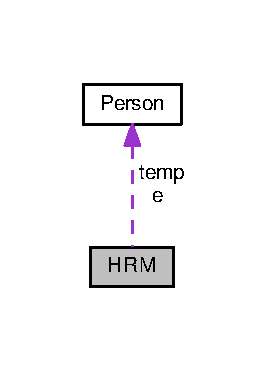
\includegraphics[width=129pt]{classHRM__coll__graph}
\end{center}
\end{figure}
\subsection*{Public Member Functions}
\begin{DoxyCompactItemize}
\item 
void \hyperlink{classHRM_ae6e340e84b8bece41f50eb138f10b6ef}{Add\+Person} ()
\item 
void \hyperlink{classHRM_ad6fd617d1fb2fccb47c7ed93aa9b9d4d}{Delete\+Person} ()
\item 
void \hyperlink{classHRM_af83289bb1e219ccf570122c689a01adc}{Search\+Person} ()
\item 
void \hyperlink{classHRM_a295019723e5d41b3cefe4982afa3f4b4}{Update\+Person} ()
\item 
void \hyperlink{classHRM_ae1fb1f404ad529d8cc690be7b8d8430e}{Report\+List} ()
\end{DoxyCompactItemize}
\subsection*{Private Attributes}
\begin{DoxyCompactItemize}
\item 
\hyperlink{classPerson}{Person} \hyperlink{classHRM_a79ccbda5f455cec5a04d53968f60e6af}{e} \mbox{[}100\mbox{]}
\item 
\hyperlink{classPerson}{Person} \hyperlink{classHRM_a6ddac0a68719ee52ed2328d0c4e6fc8f}{temp} \mbox{[}100\mbox{]}
\end{DoxyCompactItemize}


\subsection{Member Function Documentation}
\index{H\+RM@{H\+RM}!Add\+Person@{Add\+Person}}
\index{Add\+Person@{Add\+Person}!H\+RM@{H\+RM}}
\subsubsection[{\texorpdfstring{Add\+Person()}{AddPerson()}}]{\setlength{\rightskip}{0pt plus 5cm}void H\+R\+M\+::\+Add\+Person (
\begin{DoxyParamCaption}
{}
\end{DoxyParamCaption}
)}\hypertarget{classHRM_ae6e340e84b8bece41f50eb138f10b6ef}{}\label{classHRM_ae6e340e84b8bece41f50eb138f10b6ef}
\index{H\+RM@{H\+RM}!Delete\+Person@{Delete\+Person}}
\index{Delete\+Person@{Delete\+Person}!H\+RM@{H\+RM}}
\subsubsection[{\texorpdfstring{Delete\+Person()}{DeletePerson()}}]{\setlength{\rightskip}{0pt plus 5cm}void H\+R\+M\+::\+Delete\+Person (
\begin{DoxyParamCaption}
{}
\end{DoxyParamCaption}
)}\hypertarget{classHRM_ad6fd617d1fb2fccb47c7ed93aa9b9d4d}{}\label{classHRM_ad6fd617d1fb2fccb47c7ed93aa9b9d4d}
goto lebel1; 
\begin{DoxyCode}
102                        \{
103   \textcolor{comment}{//      Show all of the current employees}
104   \textcolor{comment}{//      Ask the user the ID of which employee that they wish to}
105   \textcolor{comment}{//      delete.}
106  
107   \textcolor{keywordtype}{int} empId;
108   \textcolor{keywordtype}{bool} lol;
109   \textcolor{keywordtype}{char} redo1,redo2;
110   lol =\textcolor{keyword}{false};
111 lebel:
112   cout << \textcolor{stringliteral}{"ID of employee to remove: "};
113  
114   \textcolor{keywordflow}{while}(!(cin>>empId))  \textcolor{comment}{//Reciving vaiables from input : is it no/character ?}
115   \{
116     cout << \textcolor{stringliteral}{"Please  enter a number!  Try again: "};
117     cin.clear ();
118     cin.ignore (1000, \textcolor{charliteral}{'\(\backslash\)n'});  \textcolor{comment}{// Skip to next newline or 1000 chars,}
119     \textcolor{comment}{// whichever comes first.}
120   \}
121  
122  
123  
124  
125   \textcolor{keywordflow}{for} ( \hyperlink{HumanResources_8cpp_acb559820d9ca11295b4500f179ef6392}{i} = 0; \hyperlink{HumanResources_8cpp_acb559820d9ca11295b4500f179ef6392}{i} < \hyperlink{HumanResources_8cpp_a76f11d9a0a47b94f72c2d0e77fb32240}{n}; ++\hyperlink{HumanResources_8cpp_acb559820d9ca11295b4500f179ef6392}{i}) \{
126  
127  
128     \textcolor{keywordflow}{if} (\hyperlink{HumanResources_8cpp_a76e44bc53d2efde76380be19dc9ebbc3}{y}[\hyperlink{HumanResources_8cpp_acb559820d9ca11295b4500f179ef6392}{i}]==empId) \{
129       \hyperlink{classHRM_a79ccbda5f455cec5a04d53968f60e6af}{e}[\hyperlink{HumanResources_8cpp_acb559820d9ca11295b4500f179ef6392}{i}]=\hyperlink{classHRM_a79ccbda5f455cec5a04d53968f60e6af}{e}[\hyperlink{HumanResources_8cpp_acb559820d9ca11295b4500f179ef6392}{i}+1];
130       lol=\textcolor{keyword}{true};
131       \hyperlink{classHRM_a79ccbda5f455cec5a04d53968f60e6af}{e}[\hyperlink{HumanResources_8cpp_acb559820d9ca11295b4500f179ef6392}{i}].\hyperlink{classPerson_aa78b51ba4294454e9e693b7f9a68330b}{set\_Name}();
132       cin>>redo2;
133       \textcolor{keywordflow}{if}(redo2==\textcolor{charliteral}{'Y'}||redo2==\textcolor{charliteral}{'y'})\{
134         \textcolor{keywordtype}{int} a;
135         a=\hyperlink{HumanResources_8cpp_a76f11d9a0a47b94f72c2d0e77fb32240}{n};
136  
137         cout<<\textcolor{stringliteral}{"\(\backslash\)nThe employee with the following information has been added to the system:"}<<endl;
138         cout<<\textcolor{stringliteral}{"\(\backslash\)nFirst Name       Last Name       Personal ID         Salary per year (Euros)"};
139         cout<<\textcolor{stringliteral}{"\(\backslash\)n--------------   --------------  ------------       -------------------------"}<<endl;
140         \textcolor{keywordflow}{for}(\textcolor{keywordtype}{int} \hyperlink{HumanResources_8cpp_acb559820d9ca11295b4500f179ef6392}{i}=0; \hyperlink{HumanResources_8cpp_acb559820d9ca11295b4500f179ef6392}{i}<a; \hyperlink{HumanResources_8cpp_acb559820d9ca11295b4500f179ef6392}{i}++)\{
141  
142           \hyperlink{classHRM_a79ccbda5f455cec5a04d53968f60e6af}{e}[\hyperlink{HumanResources_8cpp_acb559820d9ca11295b4500f179ef6392}{i}].\hyperlink{classPerson_a0ba48694a16ae01e279dcecca67206a1}{get\_FieldName}();
143           cout<<\textcolor{stringliteral}{"hahahahah="}<<n<<endl;
144           a--;
145           n=a;
146           n++;
147         \}
148  
149  
151       \}
152  
153       cout <<endl;
154  
155       \textcolor{comment}{//Delete function}
156     \}
157  
158   \}
159  
160  
161  
162  
163  
164   \textcolor{keywordflow}{if} (lol==\textcolor{keyword}{false}) \{
165     cout<<\textcolor{stringliteral}{"Sorry, there is not any employee with requested personal number."}
166        <<\textcolor{stringliteral}{" Do you want to repeat delete by entering the new personal number (y/n)?:"};
167     cin>>redo1;
168     \textcolor{keywordflow}{if}(redo1==\textcolor{charliteral}{'Y'}||redo1==\textcolor{charliteral}{'y'})\{
169       \textcolor{keywordflow}{goto} lebel;
170       cout<<endl<<endl;
171     \}
172   \}
173  
174  
175  
176  
177   \textcolor{comment}{//      Delete the chosen employee from the array of employees}
178   \textcolor{comment}{//      as represented in this class.}
179  
180   \textcolor{comment}{// Actually remove the entry from memory so as to not leak objects}
181   \textcolor{comment}{//nextIndex--;}
182  
183  
184 \}
\end{DoxyCode}
\index{H\+RM@{H\+RM}!Report\+List@{Report\+List}}
\index{Report\+List@{Report\+List}!H\+RM@{H\+RM}}
\subsubsection[{\texorpdfstring{Report\+List()}{ReportList()}}]{\setlength{\rightskip}{0pt plus 5cm}void H\+R\+M\+::\+Report\+List (
\begin{DoxyParamCaption}
{}
\end{DoxyParamCaption}
)}\hypertarget{classHRM_ae1fb1f404ad529d8cc690be7b8d8430e}{}\label{classHRM_ae1fb1f404ad529d8cc690be7b8d8430e}

\begin{DoxyCode}
312                      \{
313  
314   \textcolor{keywordtype}{char} op;
315   \textcolor{keywordtype}{bool} doMore;
316   cout<<\textcolor{stringliteral}{"\(\backslash\)nPlease enter the related number of the field which you would like to sort the list based on it.
      \(\backslash\)n(1. Family name, 2.Salary)?\(\backslash\)n"}<<endl;
317   \textcolor{comment}{//cin>>op;}
318   \textcolor{keywordflow}{while}(!(cin>>op))  \textcolor{comment}{//Reciving vaiables from input : is it no/character ?}
319   \{
320     cout << \textcolor{stringliteral}{"Please  enter a number!  Try again: "};
321     cin.clear ();
322     cin.ignore (1000, \textcolor{charliteral}{'\(\backslash\)n'});  \textcolor{comment}{// Skip to next newline or 1000 chars,}
323     \textcolor{comment}{// whichever comes first.}
324   \}
325  
326  
327   \textcolor{keywordflow}{switch}(op)
328   \{
329   \textcolor{keywordflow}{case} \textcolor{charliteral}{'1'}:
330     cout<<\textcolor{stringliteral}{"\(\backslash\)nSorting based on Family Name\(\backslash\)n"}<<endl;
331     \textcolor{keywordflow}{for}(\textcolor{keywordtype}{int} \hyperlink{HumanResources_8cpp_acb559820d9ca11295b4500f179ef6392}{i}=0;\hyperlink{HumanResources_8cpp_acb559820d9ca11295b4500f179ef6392}{i}<=\hyperlink{HumanResources_8cpp_a76f11d9a0a47b94f72c2d0e77fb32240}{n};\hyperlink{HumanResources_8cpp_acb559820d9ca11295b4500f179ef6392}{i}++)
332     \{
333       \textcolor{keywordflow}{for}(\textcolor{keywordtype}{int} j=\hyperlink{HumanResources_8cpp_acb559820d9ca11295b4500f179ef6392}{i}+1;j<=\hyperlink{HumanResources_8cpp_a76f11d9a0a47b94f72c2d0e77fb32240}{n}-1;j++)
334       \{
335         \textcolor{keywordflow}{if}(\hyperlink{HumanResources_8cpp_aa903d317fb89b7486b45495ea763e880}{h}[\hyperlink{HumanResources_8cpp_acb559820d9ca11295b4500f179ef6392}{i}]>\hyperlink{HumanResources_8cpp_aa903d317fb89b7486b45495ea763e880}{h}[\hyperlink{HumanResources_8cpp_acb559820d9ca11295b4500f179ef6392}{i}+1])
336         \{
337           \hyperlink{classHRM_a6ddac0a68719ee52ed2328d0c4e6fc8f}{temp}[\hyperlink{HumanResources_8cpp_acb559820d9ca11295b4500f179ef6392}{i}]=\hyperlink{classHRM_a79ccbda5f455cec5a04d53968f60e6af}{e}[\hyperlink{HumanResources_8cpp_acb559820d9ca11295b4500f179ef6392}{i}];
338           \hyperlink{classHRM_a79ccbda5f455cec5a04d53968f60e6af}{e}[\hyperlink{HumanResources_8cpp_acb559820d9ca11295b4500f179ef6392}{i}]=\hyperlink{classHRM_a79ccbda5f455cec5a04d53968f60e6af}{e}[j];
339           \hyperlink{classHRM_a79ccbda5f455cec5a04d53968f60e6af}{e}[j]=\hyperlink{classHRM_a6ddac0a68719ee52ed2328d0c4e6fc8f}{temp}[\hyperlink{HumanResources_8cpp_acb559820d9ca11295b4500f179ef6392}{i}];
340         \}
341       \}
342     \}
343  
344  
345     \textcolor{keywordflow}{for}(\textcolor{keywordtype}{int} \hyperlink{HumanResources_8cpp_acb559820d9ca11295b4500f179ef6392}{i}=0;\hyperlink{HumanResources_8cpp_acb559820d9ca11295b4500f179ef6392}{i}<\hyperlink{HumanResources_8cpp_a76f11d9a0a47b94f72c2d0e77fb32240}{n};\hyperlink{HumanResources_8cpp_acb559820d9ca11295b4500f179ef6392}{i}++)
346     \{
347       \hyperlink{classHRM_a79ccbda5f455cec5a04d53968f60e6af}{e}[\hyperlink{HumanResources_8cpp_acb559820d9ca11295b4500f179ef6392}{i}].\hyperlink{classPerson_a0ba48694a16ae01e279dcecca67206a1}{get\_FieldName}();
348     \}
349     cout<<\textcolor{stringliteral}{"\(\backslash\)nsorted\(\backslash\)n"};
350  
351     \textcolor{keywordflow}{break};
352   \textcolor{keywordflow}{case}\textcolor{charliteral}{'2'}:
353     cout<<\textcolor{stringliteral}{"\(\backslash\)nSorting based on Salary\(\backslash\)n"}<<endl;
354     \textcolor{keywordflow}{for}(\textcolor{keywordtype}{int} \hyperlink{HumanResources_8cpp_aa903d317fb89b7486b45495ea763e880}{h}=0;\hyperlink{HumanResources_8cpp_aa903d317fb89b7486b45495ea763e880}{h}<\hyperlink{HumanResources_8cpp_a76f11d9a0a47b94f72c2d0e77fb32240}{n};\hyperlink{HumanResources_8cpp_aa903d317fb89b7486b45495ea763e880}{h}++)
355     \{
356       \textcolor{keywordflow}{for}(\textcolor{keywordtype}{int} q=\hyperlink{HumanResources_8cpp_aa903d317fb89b7486b45495ea763e880}{h}+1;q<\hyperlink{HumanResources_8cpp_a76f11d9a0a47b94f72c2d0e77fb32240}{n};q++)
357       \{
358         \textcolor{keywordflow}{if}(\hyperlink{HumanResources_8cpp_ab48abf59b03ad563091fcecb765e42ab}{sal}[\hyperlink{HumanResources_8cpp_aa903d317fb89b7486b45495ea763e880}{h}]>\hyperlink{HumanResources_8cpp_ab48abf59b03ad563091fcecb765e42ab}{sal}[\hyperlink{HumanResources_8cpp_aa903d317fb89b7486b45495ea763e880}{h}+1]);
359         \{
360           \hyperlink{classHRM_a6ddac0a68719ee52ed2328d0c4e6fc8f}{temp}[\hyperlink{HumanResources_8cpp_aa903d317fb89b7486b45495ea763e880}{h}]=\hyperlink{classHRM_a79ccbda5f455cec5a04d53968f60e6af}{e}[\hyperlink{HumanResources_8cpp_aa903d317fb89b7486b45495ea763e880}{h}];
361           \hyperlink{classHRM_a79ccbda5f455cec5a04d53968f60e6af}{e}[\hyperlink{HumanResources_8cpp_aa903d317fb89b7486b45495ea763e880}{h}]=\hyperlink{classHRM_a79ccbda5f455cec5a04d53968f60e6af}{e}[q];
362           \hyperlink{classHRM_a79ccbda5f455cec5a04d53968f60e6af}{e}[q]=\hyperlink{classHRM_a6ddac0a68719ee52ed2328d0c4e6fc8f}{temp}[\hyperlink{HumanResources_8cpp_aa903d317fb89b7486b45495ea763e880}{h}];
363         \}
364       \}
365     \}
366     \textcolor{keywordflow}{for}(\textcolor{keywordtype}{int} j=0;j<\hyperlink{HumanResources_8cpp_a76f11d9a0a47b94f72c2d0e77fb32240}{n};j++)
367     \{
368       \hyperlink{classHRM_a79ccbda5f455cec5a04d53968f60e6af}{e}[j].\hyperlink{classPerson_a0ba48694a16ae01e279dcecca67206a1}{get\_FieldName}();
369     \}
370     cout<<\textcolor{stringliteral}{"\(\backslash\)nsortedlist is printed above\(\backslash\)n"};
371  
372     \textcolor{keywordflow}{break};
373   \}
374 \}
\end{DoxyCode}
\index{H\+RM@{H\+RM}!Search\+Person@{Search\+Person}}
\index{Search\+Person@{Search\+Person}!H\+RM@{H\+RM}}
\subsubsection[{\texorpdfstring{Search\+Person()}{SearchPerson()}}]{\setlength{\rightskip}{0pt plus 5cm}void H\+R\+M\+::\+Search\+Person (
\begin{DoxyParamCaption}
{}
\end{DoxyParamCaption}
)}\hypertarget{classHRM_af83289bb1e219ccf570122c689a01adc}{}\label{classHRM_af83289bb1e219ccf570122c689a01adc}

\begin{DoxyCode}
378                       \{
379   \textcolor{keywordtype}{int} c;
380   \textcolor{keywordtype}{char} redo1;
381   \textcolor{keywordtype}{string} familyname;
382   \textcolor{keywordtype}{double} min,max;
383   \textcolor{keywordflow}{do}\{
384     cout<<\textcolor{stringliteral}{"Search is based on two different fields (1.family name, 2.Salary), please enter your choice?="}<<
      endl;
385     \textcolor{comment}{//cin>>c;}
386     \textcolor{keywordflow}{while}(!(cin>>c))  \textcolor{comment}{//Reciving vaiables from input : is it no/character ?}
387     \{
388       cout << \textcolor{stringliteral}{"Please  enter a number!  Try again: "};
389       cin.clear ();
390       cin.ignore (1000, \textcolor{charliteral}{'\(\backslash\)n'});  \textcolor{comment}{// Skip to next newline or 1000 chars,}
391       \textcolor{comment}{// whichever comes first.}
392     \}
393  
394  
395     \textcolor{keywordflow}{if}(c==2)
396  
397     \{
398       cout<<\textcolor{stringliteral}{"Please define your search range for salary of employees ."}<<endl;
399       cout<<\textcolor{stringliteral}{"What is minimum salary for search (S\_min)?="}<<endl;
400       \textcolor{comment}{//cin>>min;}
401       \textcolor{keywordflow}{while}(!(cin>>min))  \textcolor{comment}{//Reciving vaiables from input : is it no/character ?}
402       \{
403         cout << \textcolor{stringliteral}{"Please  enter a number!  Try again: "};
404         cin.clear ();
405         cin.ignore (1000, \textcolor{charliteral}{'\(\backslash\)n'});  \textcolor{comment}{// Skip to next newline or 1000 chars,}
406         \textcolor{comment}{// whichever comes first.}
407       \}
408       cout<<\textcolor{stringliteral}{"What is maximum salary for search (S\_max)?="}<<endl;
409       \textcolor{comment}{//cin>>max;}
410       \textcolor{keywordflow}{while}(!(cin>>max))  \textcolor{comment}{//Reciving vaiables from input : is it no/character ?}
411       \{
412         cout << \textcolor{stringliteral}{"Please  enter a number!  Try again: "};
413         cin.clear ();
414         cin.ignore (1000, \textcolor{charliteral}{'\(\backslash\)n'});  \textcolor{comment}{// Skip to next newline or 1000 chars,}
415         \textcolor{comment}{// whichever comes first.}
416       \}
417       \textcolor{keywordtype}{int} a;
418       a=\hyperlink{HumanResources_8cpp_a76f11d9a0a47b94f72c2d0e77fb32240}{n};
419       cout<<\textcolor{stringliteral}{"\(\backslash\)nThe employee with the following information has been added to the system:"}<<endl;
420       cout<<\textcolor{stringliteral}{"\(\backslash\)nFirst Name       Last Name       Personal ID         Salary per year (Euros)"};
421       cout<<\textcolor{stringliteral}{"\(\backslash\)n--------------   --------------  ------------       -------------------------"}<<endl;
422       \textcolor{keywordflow}{for}(\textcolor{keywordtype}{int} \hyperlink{HumanResources_8cpp_acb559820d9ca11295b4500f179ef6392}{i}=0; \hyperlink{HumanResources_8cpp_acb559820d9ca11295b4500f179ef6392}{i}<\hyperlink{HumanResources_8cpp_a76f11d9a0a47b94f72c2d0e77fb32240}{n}; \hyperlink{HumanResources_8cpp_acb559820d9ca11295b4500f179ef6392}{i}++) \{
423  
424  
425         \textcolor{keywordflow}{if} (\hyperlink{HumanResources_8cpp_a2097171b622749a4748e4da254c3af72}{z}[\hyperlink{HumanResources_8cpp_acb559820d9ca11295b4500f179ef6392}{i}]>min && \hyperlink{HumanResources_8cpp_a2097171b622749a4748e4da254c3af72}{z}[\hyperlink{HumanResources_8cpp_acb559820d9ca11295b4500f179ef6392}{i}]<max) \{
426  
427           cout<<\textcolor{stringliteral}{"naaaaaaaaaaaam"}<< n<<endl;
428           \hyperlink{classHRM_a79ccbda5f455cec5a04d53968f60e6af}{e}[\hyperlink{HumanResources_8cpp_acb559820d9ca11295b4500f179ef6392}{i}].\hyperlink{classPerson_afbebe8ff11b9cf25b6df5eda1df0b447}{gett\_FieldName}();
429           cout<<\textcolor{stringliteral}{"matching="}<< \hyperlink{HumanResources_8cpp_a2097171b622749a4748e4da254c3af72}{z}[\hyperlink{HumanResources_8cpp_acb559820d9ca11295b4500f179ef6392}{i}];
430         \}
431       \}
432  
433  
434  
435     \}
436  
437     \textcolor{keywordflow}{else} \textcolor{keywordflow}{if}(c==1)
438     \{
439       cout<<\textcolor{stringliteral}{"Please enter the family name of employee?"}<<endl;
440       cin>>familyname;
441       cout<<\textcolor{stringliteral}{"\(\backslash\)nThe employee with the following information has been added to the system:"}<<endl;
442       cout<<\textcolor{stringliteral}{"\(\backslash\)nFirst Name       Last Name       Personal ID         Salary per year (Euros)"};
443       cout<<\textcolor{stringliteral}{"\(\backslash\)n--------------   --------------  ------------       -------------------------"}<<endl;
444       \textcolor{keywordflow}{for}(\textcolor{keywordtype}{int} \hyperlink{HumanResources_8cpp_acb559820d9ca11295b4500f179ef6392}{i}=0; \hyperlink{HumanResources_8cpp_acb559820d9ca11295b4500f179ef6392}{i}<\hyperlink{HumanResources_8cpp_a76f11d9a0a47b94f72c2d0e77fb32240}{n}; \hyperlink{HumanResources_8cpp_acb559820d9ca11295b4500f179ef6392}{i}++) \{
445  
446  
447         \textcolor{keywordflow}{if} (\hyperlink{HumanResources_8cpp_aa903d317fb89b7486b45495ea763e880}{h}[\hyperlink{HumanResources_8cpp_acb559820d9ca11295b4500f179ef6392}{i}]==familyname) \{
448  
449           cout<<\textcolor{stringliteral}{"naaaaaaaaaaaam"}<< n<<endl;
450           \hyperlink{classHRM_a79ccbda5f455cec5a04d53968f60e6af}{e}[\hyperlink{HumanResources_8cpp_acb559820d9ca11295b4500f179ef6392}{i}].\hyperlink{classPerson_afbebe8ff11b9cf25b6df5eda1df0b447}{gett\_FieldName}();
451           cout<<\textcolor{stringliteral}{"matching="}<< \hyperlink{HumanResources_8cpp_a2097171b622749a4748e4da254c3af72}{z}[\hyperlink{HumanResources_8cpp_acb559820d9ca11295b4500f179ef6392}{i}];
452         \}
453       \}
454     \}
455  
456     cout<<\textcolor{stringliteral}{"\(\backslash\)nDo you want to Search any other field (y/n)?\(\backslash\)n"}<<endl;
457     cin>>redo1;
458   \}\textcolor{keywordflow}{while}(redo1==\textcolor{charliteral}{'y'}||redo1==\textcolor{charliteral}{'Y'});
459  
460  
461 \}
\end{DoxyCode}
\index{H\+RM@{H\+RM}!Update\+Person@{Update\+Person}}
\index{Update\+Person@{Update\+Person}!H\+RM@{H\+RM}}
\subsubsection[{\texorpdfstring{Update\+Person()}{UpdatePerson()}}]{\setlength{\rightskip}{0pt plus 5cm}void H\+R\+M\+::\+Update\+Person (
\begin{DoxyParamCaption}
{}
\end{DoxyParamCaption}
)}\hypertarget{classHRM_a295019723e5d41b3cefe4982afa3f4b4}{}\label{classHRM_a295019723e5d41b3cefe4982afa3f4b4}

\begin{DoxyCode}
190                       \{
191  
192   \textcolor{keywordtype}{int} empId;
193   \textcolor{keywordtype}{char} redo1,redo2;
194  
195 lebel:
196   cout << \textcolor{stringliteral}{"ID of employee to modify data: "};
197  
198   \textcolor{keywordflow}{while}(!(cin>>empId))  \textcolor{comment}{//Reciving vaiables from input : is it no/character ?}
199   \{
200     cout << \textcolor{stringliteral}{"Please  enter a number!  Try again: "};
201     cin.clear ();
202     cin.ignore (1000, \textcolor{charliteral}{'\(\backslash\)n'});  \textcolor{comment}{// Skip to next newline or 1000 chars,}
203     \textcolor{comment}{// whichever comes first.}
204   \}
205  
206  
207  
208  
209   \textcolor{keywordtype}{int} flag1=0;
210   \textcolor{keywordflow}{for} (\textcolor{keywordtype}{int} \hyperlink{HumanResources_8cpp_acb559820d9ca11295b4500f179ef6392}{i} = 0; \hyperlink{HumanResources_8cpp_acb559820d9ca11295b4500f179ef6392}{i} < \hyperlink{HumanResources_8cpp_a76f11d9a0a47b94f72c2d0e77fb32240}{n}; ++\hyperlink{HumanResources_8cpp_acb559820d9ca11295b4500f179ef6392}{i}) \{
211  
212     \textcolor{keywordflow}{if} (\hyperlink{HumanResources_8cpp_a76e44bc53d2efde76380be19dc9ebbc3}{y}[\hyperlink{HumanResources_8cpp_acb559820d9ca11295b4500f179ef6392}{i}]!=empId) \{
213       flag1++;
214  
215     \}
216   \}
217   \textcolor{comment}{/*  if (flag1==n)\{}
218 \textcolor{comment}{ }
219 \textcolor{comment}{                         // cout<<" not     matching="<< y[i];}
220 \textcolor{comment}{cout<<"Sorry, there is not any employee with requested personal number. Do you want to repeat delete by
       entering the new personal number (y/n)?:";}
221 \textcolor{comment}{                     cin>>redo1;}
222 \textcolor{comment}{                          if(redo1=='Y'||redo1=='y')\{}
223 \textcolor{comment}{                          goto lebel;}
224 \textcolor{comment}{                            \}}
225 \textcolor{comment}{                          \} */}
226  
227   cout <<endl;
228 lebel1:
229  
230   \textcolor{keywordflow}{for} (\textcolor{keywordtype}{int} \hyperlink{HumanResources_8cpp_acb559820d9ca11295b4500f179ef6392}{i} = 0; \hyperlink{HumanResources_8cpp_acb559820d9ca11295b4500f179ef6392}{i} < \hyperlink{HumanResources_8cpp_a76f11d9a0a47b94f72c2d0e77fb32240}{n}; ++\hyperlink{HumanResources_8cpp_acb559820d9ca11295b4500f179ef6392}{i}) \{
231  
232  
233     \textcolor{keywordflow}{if} (\hyperlink{HumanResources_8cpp_a76e44bc53d2efde76380be19dc9ebbc3}{y}[\hyperlink{HumanResources_8cpp_acb559820d9ca11295b4500f179ef6392}{i}]==empId) \{
234  
235       cout<<\textcolor{stringliteral}{"matching="}<< \hyperlink{HumanResources_8cpp_a76e44bc53d2efde76380be19dc9ebbc3}{y}[\hyperlink{HumanResources_8cpp_acb559820d9ca11295b4500f179ef6392}{i}];
236  
237       \hyperlink{HumanResources_8cpp_a8b3ab54ed3e81c69863d65e4e6c424a0}{flag}=\textcolor{keyword}{true};
238       \textcolor{keywordtype}{int} choice = 0;
239       \textcolor{keywordtype}{char} redo;
240  
241       \textcolor{keywordflow}{do} \{
242         cout << endl << endl;
243         cout << \textcolor{stringliteral}{"Please enter the related number of field which you would like to update"} << endl;
244         cout <<\textcolor{stringliteral}{"1. First name"} << endl;
245         cout << \textcolor{stringliteral}{"2. Family name"} << endl;
246         cout << \textcolor{stringliteral}{"3. Working hours per week"} << endl;
247         cout << \textcolor{stringliteral}{"4. Payment for one hour"} << endl;
248         cout << std::endl;
249  
250         cin >> choice;
251         \textcolor{keywordflow}{if} (choice == 1) \{
252           cout << \textcolor{stringliteral}{" First name: "};
253           \hyperlink{classHRM_a79ccbda5f455cec5a04d53968f60e6af}{e}[\hyperlink{HumanResources_8cpp_acb559820d9ca11295b4500f179ef6392}{i}].\hyperlink{classPerson_a07320273da2b8a6957300d20d4594195}{in\_FirstName}();
254         \}
255         \textcolor{keywordflow}{else} \textcolor{keywordflow}{if} (choice == 2) \{
256           cout << \textcolor{stringliteral}{" Family name: "};
257           \hyperlink{classHRM_a79ccbda5f455cec5a04d53968f60e6af}{e}[\hyperlink{HumanResources_8cpp_acb559820d9ca11295b4500f179ef6392}{i}].\hyperlink{classPerson_a7ebc969ff71b7a9f93ff1e88a94c78d2}{in\_FamilyName}();
258         \}
259         \textcolor{keywordflow}{else} \textcolor{keywordflow}{if} (choice == 3) \{
260           cout << \textcolor{stringliteral}{" Working hours per week: "};
261           \hyperlink{classHRM_a79ccbda5f455cec5a04d53968f60e6af}{e}[\hyperlink{HumanResources_8cpp_acb559820d9ca11295b4500f179ef6392}{i}].\hyperlink{classPerson_a1aac8b7a7c6fa6c4ed3c7ce96d98c65e}{in\_Workinghour}();
262         \}
263         \textcolor{keywordflow}{else} \textcolor{keywordflow}{if} (choice == 4) \{
264           cout << \textcolor{stringliteral}{" Payment for one hour: "};
265           \hyperlink{classHRM_a79ccbda5f455cec5a04d53968f60e6af}{e}[\hyperlink{HumanResources_8cpp_acb559820d9ca11295b4500f179ef6392}{i}].\hyperlink{classPerson_a81602e50aff78c8f2d8eef65f422388a}{in\_Costperhour}();
266         \}
267         cout<<\textcolor{stringliteral}{"Do you want to update another field (Y/N)="};
268         cin>>redo;
269       \} \textcolor{keywordflow}{while} (redo==\textcolor{charliteral}{'y'}||redo==\textcolor{charliteral}{'Y'});
270     \}
271   \}
272   \textcolor{keywordtype}{int} a;
273   a=\hyperlink{HumanResources_8cpp_a76f11d9a0a47b94f72c2d0e77fb32240}{n};
274   cout<<\textcolor{stringliteral}{"\(\backslash\)nThe employee with the following information has been added to the system:"}<<endl;
275   cout<<\textcolor{stringliteral}{"\(\backslash\)nFirst Name       Last Name       Personal ID         Salary per year (Euros)"};
276   cout<<\textcolor{stringliteral}{"\(\backslash\)n--------------   --------------  ------------       -------------------------"}<<endl;
277   \textcolor{keywordflow}{for}(\textcolor{keywordtype}{int} \hyperlink{HumanResources_8cpp_acb559820d9ca11295b4500f179ef6392}{i}=0; \hyperlink{HumanResources_8cpp_acb559820d9ca11295b4500f179ef6392}{i}<a; \hyperlink{HumanResources_8cpp_acb559820d9ca11295b4500f179ef6392}{i}++)\{
278     \hyperlink{classHRM_a79ccbda5f455cec5a04d53968f60e6af}{e}[\hyperlink{HumanResources_8cpp_acb559820d9ca11295b4500f179ef6392}{i}].\hyperlink{classPerson_a0ba48694a16ae01e279dcecca67206a1}{get\_FieldName}();
279  
280     cout<<\textcolor{stringliteral}{"hahahahah="}<<n<<endl;
281  
282   \}
283 \}
\end{DoxyCode}


\subsection{Member Data Documentation}
\index{H\+RM@{H\+RM}!e@{e}}
\index{e@{e}!H\+RM@{H\+RM}}
\subsubsection[{\texorpdfstring{e}{e}}]{\setlength{\rightskip}{0pt plus 5cm}{\bf Person} H\+R\+M\+::e\mbox{[}100\mbox{]}\hspace{0.3cm}{\ttfamily [private]}}\hypertarget{classHRM_a79ccbda5f455cec5a04d53968f60e6af}{}\label{classHRM_a79ccbda5f455cec5a04d53968f60e6af}
\index{H\+RM@{H\+RM}!temp@{temp}}
\index{temp@{temp}!H\+RM@{H\+RM}}
\subsubsection[{\texorpdfstring{temp}{temp}}]{\setlength{\rightskip}{0pt plus 5cm}{\bf Person} H\+R\+M\+::temp\mbox{[}100\mbox{]}\hspace{0.3cm}{\ttfamily [private]}}\hypertarget{classHRM_a6ddac0a68719ee52ed2328d0c4e6fc8f}{}\label{classHRM_a6ddac0a68719ee52ed2328d0c4e6fc8f}


The documentation for this class was generated from the following file\+:\begin{DoxyCompactItemize}
\item 
\hyperlink{HumanResources_8cpp}{Human\+Resources.\+cpp}\end{DoxyCompactItemize}

\hypertarget{classPerson}{}\section{Person Class Reference}
\label{classPerson}\index{Person@{Person}}
\subsection*{Public Member Functions}
\begin{DoxyCompactItemize}
\item 
void \hyperlink{classPerson_a3abd7c29b92129b97a4f1000cced9c51}{set\+\_\+\+Field\+Name} ()
\item 
void \hyperlink{classPerson_a0ba48694a16ae01e279dcecca67206a1}{get\+\_\+\+Field\+Name} ()
\item 
void \hyperlink{classPerson_afbebe8ff11b9cf25b6df5eda1df0b447}{gett\+\_\+\+Field\+Name} ()
\item 
void \hyperlink{classPerson_a3d43cd58a6006f81794caa94c07810d6}{set\+\_\+\+Personal\+ID} ()
\item 
void \hyperlink{classPerson_aa78b51ba4294454e9e693b7f9a68330b}{set\+\_\+\+Name} ()
\item 
void \hyperlink{classPerson_aa31e49027355ebe88555ed25144edd24}{Last\+Namesort\+List} ()
\item 
void \hyperlink{classPerson_a07320273da2b8a6957300d20d4594195}{in\+\_\+\+First\+Name} ()
\item 
void \hyperlink{classPerson_a7ebc969ff71b7a9f93ff1e88a94c78d2}{in\+\_\+\+Family\+Name} ()
\item 
void \hyperlink{classPerson_a1aac8b7a7c6fa6c4ed3c7ce96d98c65e}{in\+\_\+\+Workinghour} ()
\item 
void \hyperlink{classPerson_a81602e50aff78c8f2d8eef65f422388a}{in\+\_\+\+Costperhour} ()
\end{DoxyCompactItemize}
\subsection*{Private Attributes}
\begin{DoxyCompactItemize}
\item 
string \hyperlink{classPerson_aa7e415d2232d63bebe953227394bdf02}{First\+Name}
\item 
string \hyperlink{classPerson_adb7b4b0c1c6d35ff77be67f36bfae396}{Last\+Name}
\item 
int \hyperlink{classPerson_a4e13ba0eb54b26b2ef7b18022e609edb}{Personal\+ID}
\item 
double \hyperlink{classPerson_a096ebbbd6a4a7552bf385aa67e379345}{Salary}
\item 
double \hyperlink{classPerson_aadb5de5c82650fdfa71c51caada68e4f}{Working\+Hours}
\item 
double \hyperlink{classPerson_a7ac09228195bedb1247a9d070de63dfe}{Cost\+Per\+Hour}
\end{DoxyCompactItemize}


\subsection{Member Function Documentation}
\index{Person@{Person}!get\+\_\+\+Field\+Name@{get\+\_\+\+Field\+Name}}
\index{get\+\_\+\+Field\+Name@{get\+\_\+\+Field\+Name}!Person@{Person}}
\subsubsection[{\texorpdfstring{get\+\_\+\+Field\+Name()}{get_FieldName()}}]{\setlength{\rightskip}{0pt plus 5cm}void Person\+::get\+\_\+\+Field\+Name (
\begin{DoxyParamCaption}
{}
\end{DoxyParamCaption}
)}\hypertarget{classPerson_a0ba48694a16ae01e279dcecca67206a1}{}\label{classPerson_a0ba48694a16ae01e279dcecca67206a1}
\index{Person@{Person}!gett\+\_\+\+Field\+Name@{gett\+\_\+\+Field\+Name}}
\index{gett\+\_\+\+Field\+Name@{gett\+\_\+\+Field\+Name}!Person@{Person}}
\subsubsection[{\texorpdfstring{gett\+\_\+\+Field\+Name()}{gett_FieldName()}}]{\setlength{\rightskip}{0pt plus 5cm}void Person\+::gett\+\_\+\+Field\+Name (
\begin{DoxyParamCaption}
{}
\end{DoxyParamCaption}
)}\hypertarget{classPerson_afbebe8ff11b9cf25b6df5eda1df0b447}{}\label{classPerson_afbebe8ff11b9cf25b6df5eda1df0b447}
\index{Person@{Person}!in\+\_\+\+Costperhour@{in\+\_\+\+Costperhour}}
\index{in\+\_\+\+Costperhour@{in\+\_\+\+Costperhour}!Person@{Person}}
\subsubsection[{\texorpdfstring{in\+\_\+\+Costperhour()}{in_Costperhour()}}]{\setlength{\rightskip}{0pt plus 5cm}void Person\+::in\+\_\+\+Costperhour (
\begin{DoxyParamCaption}
{}
\end{DoxyParamCaption}
)}\hypertarget{classPerson_a81602e50aff78c8f2d8eef65f422388a}{}\label{classPerson_a81602e50aff78c8f2d8eef65f422388a}
\index{Person@{Person}!in\+\_\+\+Family\+Name@{in\+\_\+\+Family\+Name}}
\index{in\+\_\+\+Family\+Name@{in\+\_\+\+Family\+Name}!Person@{Person}}
\subsubsection[{\texorpdfstring{in\+\_\+\+Family\+Name()}{in_FamilyName()}}]{\setlength{\rightskip}{0pt plus 5cm}void Person\+::in\+\_\+\+Family\+Name (
\begin{DoxyParamCaption}
{}
\end{DoxyParamCaption}
)}\hypertarget{classPerson_a7ebc969ff71b7a9f93ff1e88a94c78d2}{}\label{classPerson_a7ebc969ff71b7a9f93ff1e88a94c78d2}
\index{Person@{Person}!in\+\_\+\+First\+Name@{in\+\_\+\+First\+Name}}
\index{in\+\_\+\+First\+Name@{in\+\_\+\+First\+Name}!Person@{Person}}
\subsubsection[{\texorpdfstring{in\+\_\+\+First\+Name()}{in_FirstName()}}]{\setlength{\rightskip}{0pt plus 5cm}void Person\+::in\+\_\+\+First\+Name (
\begin{DoxyParamCaption}
{}
\end{DoxyParamCaption}
)}\hypertarget{classPerson_a07320273da2b8a6957300d20d4594195}{}\label{classPerson_a07320273da2b8a6957300d20d4594195}
\index{Person@{Person}!in\+\_\+\+Workinghour@{in\+\_\+\+Workinghour}}
\index{in\+\_\+\+Workinghour@{in\+\_\+\+Workinghour}!Person@{Person}}
\subsubsection[{\texorpdfstring{in\+\_\+\+Workinghour()}{in_Workinghour()}}]{\setlength{\rightskip}{0pt plus 5cm}void Person\+::in\+\_\+\+Workinghour (
\begin{DoxyParamCaption}
{}
\end{DoxyParamCaption}
)}\hypertarget{classPerson_a1aac8b7a7c6fa6c4ed3c7ce96d98c65e}{}\label{classPerson_a1aac8b7a7c6fa6c4ed3c7ce96d98c65e}
\index{Person@{Person}!Last\+Namesort\+List@{Last\+Namesort\+List}}
\index{Last\+Namesort\+List@{Last\+Namesort\+List}!Person@{Person}}
\subsubsection[{\texorpdfstring{Last\+Namesort\+List()}{LastNamesortList()}}]{\setlength{\rightskip}{0pt plus 5cm}void Person\+::\+Last\+Namesort\+List (
\begin{DoxyParamCaption}
{}
\end{DoxyParamCaption}
)}\hypertarget{classPerson_aa31e49027355ebe88555ed25144edd24}{}\label{classPerson_aa31e49027355ebe88555ed25144edd24}
\index{Person@{Person}!set\+\_\+\+Field\+Name@{set\+\_\+\+Field\+Name}}
\index{set\+\_\+\+Field\+Name@{set\+\_\+\+Field\+Name}!Person@{Person}}
\subsubsection[{\texorpdfstring{set\+\_\+\+Field\+Name()}{set_FieldName()}}]{\setlength{\rightskip}{0pt plus 5cm}void Person\+::set\+\_\+\+Field\+Name (
\begin{DoxyParamCaption}
{}
\end{DoxyParamCaption}
)}\hypertarget{classPerson_a3abd7c29b92129b97a4f1000cced9c51}{}\label{classPerson_a3abd7c29b92129b97a4f1000cced9c51}
\index{Person@{Person}!set\+\_\+\+Name@{set\+\_\+\+Name}}
\index{set\+\_\+\+Name@{set\+\_\+\+Name}!Person@{Person}}
\subsubsection[{\texorpdfstring{set\+\_\+\+Name()}{set_Name()}}]{\setlength{\rightskip}{0pt plus 5cm}void Person\+::set\+\_\+\+Name (
\begin{DoxyParamCaption}
{}
\end{DoxyParamCaption}
)}\hypertarget{classPerson_aa78b51ba4294454e9e693b7f9a68330b}{}\label{classPerson_aa78b51ba4294454e9e693b7f9a68330b}
\index{Person@{Person}!set\+\_\+\+Personal\+ID@{set\+\_\+\+Personal\+ID}}
\index{set\+\_\+\+Personal\+ID@{set\+\_\+\+Personal\+ID}!Person@{Person}}
\subsubsection[{\texorpdfstring{set\+\_\+\+Personal\+I\+D()}{set_PersonalID()}}]{\setlength{\rightskip}{0pt plus 5cm}void Person\+::set\+\_\+\+Personal\+ID (
\begin{DoxyParamCaption}
{}
\end{DoxyParamCaption}
)}\hypertarget{classPerson_a3d43cd58a6006f81794caa94c07810d6}{}\label{classPerson_a3d43cd58a6006f81794caa94c07810d6}


\subsection{Member Data Documentation}
\index{Person@{Person}!Cost\+Per\+Hour@{Cost\+Per\+Hour}}
\index{Cost\+Per\+Hour@{Cost\+Per\+Hour}!Person@{Person}}
\subsubsection[{\texorpdfstring{Cost\+Per\+Hour}{CostPerHour}}]{\setlength{\rightskip}{0pt plus 5cm}double Person\+::\+Cost\+Per\+Hour\hspace{0.3cm}{\ttfamily [private]}}\hypertarget{classPerson_a7ac09228195bedb1247a9d070de63dfe}{}\label{classPerson_a7ac09228195bedb1247a9d070de63dfe}
\index{Person@{Person}!First\+Name@{First\+Name}}
\index{First\+Name@{First\+Name}!Person@{Person}}
\subsubsection[{\texorpdfstring{First\+Name}{FirstName}}]{\setlength{\rightskip}{0pt plus 5cm}string Person\+::\+First\+Name\hspace{0.3cm}{\ttfamily [private]}}\hypertarget{classPerson_aa7e415d2232d63bebe953227394bdf02}{}\label{classPerson_aa7e415d2232d63bebe953227394bdf02}
\index{Person@{Person}!Last\+Name@{Last\+Name}}
\index{Last\+Name@{Last\+Name}!Person@{Person}}
\subsubsection[{\texorpdfstring{Last\+Name}{LastName}}]{\setlength{\rightskip}{0pt plus 5cm}string Person\+::\+Last\+Name\hspace{0.3cm}{\ttfamily [private]}}\hypertarget{classPerson_adb7b4b0c1c6d35ff77be67f36bfae396}{}\label{classPerson_adb7b4b0c1c6d35ff77be67f36bfae396}
\index{Person@{Person}!Personal\+ID@{Personal\+ID}}
\index{Personal\+ID@{Personal\+ID}!Person@{Person}}
\subsubsection[{\texorpdfstring{Personal\+ID}{PersonalID}}]{\setlength{\rightskip}{0pt plus 5cm}int Person\+::\+Personal\+ID\hspace{0.3cm}{\ttfamily [private]}}\hypertarget{classPerson_a4e13ba0eb54b26b2ef7b18022e609edb}{}\label{classPerson_a4e13ba0eb54b26b2ef7b18022e609edb}
\index{Person@{Person}!Salary@{Salary}}
\index{Salary@{Salary}!Person@{Person}}
\subsubsection[{\texorpdfstring{Salary}{Salary}}]{\setlength{\rightskip}{0pt plus 5cm}double Person\+::\+Salary\hspace{0.3cm}{\ttfamily [private]}}\hypertarget{classPerson_a096ebbbd6a4a7552bf385aa67e379345}{}\label{classPerson_a096ebbbd6a4a7552bf385aa67e379345}
\index{Person@{Person}!Working\+Hours@{Working\+Hours}}
\index{Working\+Hours@{Working\+Hours}!Person@{Person}}
\subsubsection[{\texorpdfstring{Working\+Hours}{WorkingHours}}]{\setlength{\rightskip}{0pt plus 5cm}double Person\+::\+Working\+Hours\hspace{0.3cm}{\ttfamily [private]}}\hypertarget{classPerson_aadb5de5c82650fdfa71c51caada68e4f}{}\label{classPerson_aadb5de5c82650fdfa71c51caada68e4f}


The documentation for this class was generated from the following file\+:\begin{DoxyCompactItemize}
\item 
\hyperlink{HumanResources_8cpp}{Human\+Resources.\+cpp}\end{DoxyCompactItemize}

\chapter{File Documentation}
\hypertarget{HumanResources_8cpp}{}\section{Human\+Resources.\+cpp File Reference}
\label{HumanResources_8cpp}\index{Human\+Resources.\+cpp@{Human\+Resources.\+cpp}}
{\ttfamily \#include $<$iostream$>$}\\*
{\ttfamily \#include $<$math.\+h$>$}\\*
{\ttfamily \#include $<$cstdlib$>$}\\*
{\ttfamily \#include $<$string$>$}\\*
Include dependency graph for Human\+Resources.\+cpp\+:
\nopagebreak
\begin{figure}[H]
\begin{center}
\leavevmode
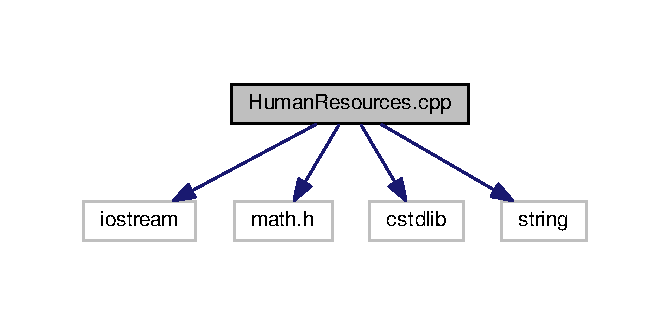
\includegraphics[width=322pt]{HumanResources_8cpp__incl}
\end{center}
\end{figure}
\subsection*{Classes}
\begin{DoxyCompactItemize}
\item 
class \hyperlink{classPerson}{Person}
\item 
class \hyperlink{classHRM}{H\+RM}
\end{DoxyCompactItemize}
\subsection*{Functions}
\begin{DoxyCompactItemize}
\item 
int \hyperlink{HumanResources_8cpp_ae66f6b31b5ad750f1fe042a706a4e3d4}{main} ()
\end{DoxyCompactItemize}
\subsection*{Variables}
\begin{DoxyCompactItemize}
\item 
int \hyperlink{HumanResources_8cpp_a76f11d9a0a47b94f72c2d0e77fb32240}{n} =0
\item 
int \hyperlink{HumanResources_8cpp_acb559820d9ca11295b4500f179ef6392}{i} =0
\item 
int \hyperlink{HumanResources_8cpp_a6150e0515f7202e2fb518f7206ed97dc}{x} =8248001
\item 
int \hyperlink{HumanResources_8cpp_a76e44bc53d2efde76380be19dc9ebbc3}{y} \mbox{[}100\mbox{]}
\item 
bool \hyperlink{HumanResources_8cpp_a8b3ab54ed3e81c69863d65e4e6c424a0}{flag} =0
\item 
int \hyperlink{HumanResources_8cpp_a2097171b622749a4748e4da254c3af72}{z} \mbox{[}100\mbox{]}
\item 
string \hyperlink{HumanResources_8cpp_aa903d317fb89b7486b45495ea763e880}{h} \mbox{[}100\mbox{]}
\item 
double \hyperlink{HumanResources_8cpp_ab48abf59b03ad563091fcecb765e42ab}{sal} \mbox{[}100\mbox{]}
\item 
int \hyperlink{HumanResources_8cpp_a5aa1731610537e057191db627c19f1ca}{check} =0
\item 
int \hyperlink{HumanResources_8cpp_ab66ed8e0098c0a86b458672a55a9cca9}{k} =0
\end{DoxyCompactItemize}


\subsection{Function Documentation}
\index{Human\+Resources.\+cpp@{Human\+Resources.\+cpp}!main@{main}}
\index{main@{main}!Human\+Resources.\+cpp@{Human\+Resources.\+cpp}}
\subsubsection[{\texorpdfstring{main()}{main()}}]{\setlength{\rightskip}{0pt plus 5cm}int main (
\begin{DoxyParamCaption}
{}
\end{DoxyParamCaption}
)}\hypertarget{HumanResources_8cpp_ae66f6b31b5ad750f1fe042a706a4e3d4}{}\label{HumanResources_8cpp_ae66f6b31b5ad750f1fe042a706a4e3d4}

\begin{DoxyCode}
539 \{
540   \textcolor{comment}{//-------defining variables and initializing them-------------}
541  
542  
543   \hyperlink{classHRM}{HRM} info ;
544  
545   \textcolor{keywordtype}{int} c;
546   \textcolor{keywordtype}{char} operation,ch;
547   \textcolor{comment}{//--------Printing my name on screen----------------}
548   cout<<        \textcolor{stringliteral}{"Welcome to the  program 2.1 written by Your Name"}<<endl;
549   cout<<\textcolor{stringliteral}{"**************************************************************************"}<<endl;
550   cout<<endl<<endl<<endl;
551   \textcolor{keywordflow}{do}
552   \{
553  
554     cout<<\textcolor{stringliteral}{"Welcome to Human Resource Management (HRM) Software of Company XYZ."};
555     cout<<\textcolor{stringliteral}{"To do specific task please choose one of the following commands."}<<endl<<endl<<endl;
556     cout<<\textcolor{stringliteral}{"    1. Add new employee"}<<endl;
557     cout<<\textcolor{stringliteral}{"    2. Delete employee information"}<<endl;
558     cout<<\textcolor{stringliteral}{"    3. Update employee information"}<<endl;
559     cout<<\textcolor{stringliteral}{"    4. Make reports based on specific field"}<<endl;
560     cout<<\textcolor{stringliteral}{"    5. Search employee"}<<endl;
561     cout<<\textcolor{stringliteral}{"    6. Quit"}<<endl<<endl;
562  
563  
564     \textcolor{keywordflow}{while}(!(cin>>c))  \textcolor{comment}{//Reciving vaiables from input : is it no/character ?}
565     \{
566       cout << \textcolor{stringliteral}{"Please  enter a number!  Try again: "};
567       cin.clear ();
568       cin.ignore (1000, \textcolor{charliteral}{'\(\backslash\)n'});  \textcolor{comment}{// Skip to next newline or 1000 chars,}
569       \textcolor{comment}{// whichever comes first.}
570     \}
571     \textcolor{keywordflow}{switch}(c)
572     \{
573     \textcolor{keywordflow}{case} 1:
574       cout<<\textcolor{stringliteral}{"\(\backslash\)nEnter the information of the new employee"}<<endl;
575       info.\hyperlink{classHRM_ae6e340e84b8bece41f50eb138f10b6ef}{AddPerson}();
576       \textcolor{keywordflow}{break};
577     \textcolor{keywordflow}{case} 2:
578       info.\hyperlink{classHRM_ad6fd617d1fb2fccb47c7ed93aa9b9d4d}{DeletePerson}();
579       \textcolor{keywordflow}{break};
580     \textcolor{keywordflow}{case} 3:
581       cout<<\textcolor{stringliteral}{"\(\backslash\)nEnter an item to deletion"};
582       info.\hyperlink{classHRM_a295019723e5d41b3cefe4982afa3f4b4}{UpdatePerson}();
583       \textcolor{keywordflow}{break};
584     \textcolor{keywordflow}{case} 4:
585       cout<<\textcolor{stringliteral}{"\(\backslash\)nEnter an element to search"};
586       info.\hyperlink{classHRM_ae1fb1f404ad529d8cc690be7b8d8430e}{ReportList}();
587       \textcolor{keywordflow}{break};
588     \textcolor{keywordflow}{case} 5:
589       info.\hyperlink{classHRM_af83289bb1e219ccf570122c689a01adc}{SearchPerson}();
590       \textcolor{keywordflow}{break};
591     \textcolor{keywordflow}{default} :
592       cout<<\textcolor{stringliteral}{"\(\backslash\)nInvalid option try again"};
593  
594     \}
595     cout<<\textcolor{stringliteral}{"\(\backslash\)ndo u want to continue"};
596     cin>>ch;
597   \}
598   \textcolor{keywordflow}{while}(ch==\textcolor{charliteral}{'y'}||ch==\textcolor{charliteral}{'Y'});
599  
600  
601   system(\textcolor{stringliteral}{"pause"});
602   \textcolor{keywordflow}{return} 0;
603 \}\end{DoxyCode}


Here is the call graph for this function\+:
\nopagebreak
\begin{figure}[H]
\begin{center}
\leavevmode
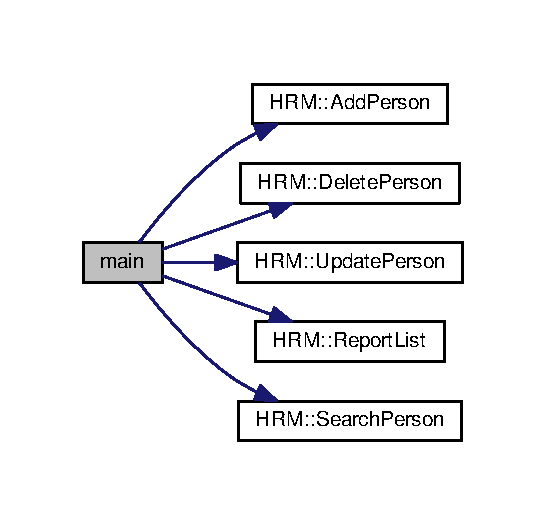
\includegraphics[width=262pt]{HumanResources_8cpp_ae66f6b31b5ad750f1fe042a706a4e3d4_cgraph}
\end{center}
\end{figure}




\subsection{Variable Documentation}
\index{Human\+Resources.\+cpp@{Human\+Resources.\+cpp}!check@{check}}
\index{check@{check}!Human\+Resources.\+cpp@{Human\+Resources.\+cpp}}
\subsubsection[{\texorpdfstring{check}{check}}]{\setlength{\rightskip}{0pt plus 5cm}int check =0}\hypertarget{HumanResources_8cpp_a5aa1731610537e057191db627c19f1ca}{}\label{HumanResources_8cpp_a5aa1731610537e057191db627c19f1ca}
\index{Human\+Resources.\+cpp@{Human\+Resources.\+cpp}!flag@{flag}}
\index{flag@{flag}!Human\+Resources.\+cpp@{Human\+Resources.\+cpp}}
\subsubsection[{\texorpdfstring{flag}{flag}}]{\setlength{\rightskip}{0pt plus 5cm}bool flag =0}\hypertarget{HumanResources_8cpp_a8b3ab54ed3e81c69863d65e4e6c424a0}{}\label{HumanResources_8cpp_a8b3ab54ed3e81c69863d65e4e6c424a0}
\index{Human\+Resources.\+cpp@{Human\+Resources.\+cpp}!h@{h}}
\index{h@{h}!Human\+Resources.\+cpp@{Human\+Resources.\+cpp}}
\subsubsection[{\texorpdfstring{h}{h}}]{\setlength{\rightskip}{0pt plus 5cm}string h\mbox{[}100\mbox{]}}\hypertarget{HumanResources_8cpp_aa903d317fb89b7486b45495ea763e880}{}\label{HumanResources_8cpp_aa903d317fb89b7486b45495ea763e880}
\index{Human\+Resources.\+cpp@{Human\+Resources.\+cpp}!i@{i}}
\index{i@{i}!Human\+Resources.\+cpp@{Human\+Resources.\+cpp}}
\subsubsection[{\texorpdfstring{i}{i}}]{\setlength{\rightskip}{0pt plus 5cm}int i =0}\hypertarget{HumanResources_8cpp_acb559820d9ca11295b4500f179ef6392}{}\label{HumanResources_8cpp_acb559820d9ca11295b4500f179ef6392}
\index{Human\+Resources.\+cpp@{Human\+Resources.\+cpp}!k@{k}}
\index{k@{k}!Human\+Resources.\+cpp@{Human\+Resources.\+cpp}}
\subsubsection[{\texorpdfstring{k}{k}}]{\setlength{\rightskip}{0pt plus 5cm}int k =0}\hypertarget{HumanResources_8cpp_ab66ed8e0098c0a86b458672a55a9cca9}{}\label{HumanResources_8cpp_ab66ed8e0098c0a86b458672a55a9cca9}
\index{Human\+Resources.\+cpp@{Human\+Resources.\+cpp}!n@{n}}
\index{n@{n}!Human\+Resources.\+cpp@{Human\+Resources.\+cpp}}
\subsubsection[{\texorpdfstring{n}{n}}]{\setlength{\rightskip}{0pt plus 5cm}int n =0}\hypertarget{HumanResources_8cpp_a76f11d9a0a47b94f72c2d0e77fb32240}{}\label{HumanResources_8cpp_a76f11d9a0a47b94f72c2d0e77fb32240}
\index{Human\+Resources.\+cpp@{Human\+Resources.\+cpp}!sal@{sal}}
\index{sal@{sal}!Human\+Resources.\+cpp@{Human\+Resources.\+cpp}}
\subsubsection[{\texorpdfstring{sal}{sal}}]{\setlength{\rightskip}{0pt plus 5cm}double sal\mbox{[}100\mbox{]}}\hypertarget{HumanResources_8cpp_ab48abf59b03ad563091fcecb765e42ab}{}\label{HumanResources_8cpp_ab48abf59b03ad563091fcecb765e42ab}
\index{Human\+Resources.\+cpp@{Human\+Resources.\+cpp}!x@{x}}
\index{x@{x}!Human\+Resources.\+cpp@{Human\+Resources.\+cpp}}
\subsubsection[{\texorpdfstring{x}{x}}]{\setlength{\rightskip}{0pt plus 5cm}int x =8248001}\hypertarget{HumanResources_8cpp_a6150e0515f7202e2fb518f7206ed97dc}{}\label{HumanResources_8cpp_a6150e0515f7202e2fb518f7206ed97dc}
\index{Human\+Resources.\+cpp@{Human\+Resources.\+cpp}!y@{y}}
\index{y@{y}!Human\+Resources.\+cpp@{Human\+Resources.\+cpp}}
\subsubsection[{\texorpdfstring{y}{y}}]{\setlength{\rightskip}{0pt plus 5cm}int y\mbox{[}100\mbox{]}}\hypertarget{HumanResources_8cpp_a76e44bc53d2efde76380be19dc9ebbc3}{}\label{HumanResources_8cpp_a76e44bc53d2efde76380be19dc9ebbc3}
\index{Human\+Resources.\+cpp@{Human\+Resources.\+cpp}!z@{z}}
\index{z@{z}!Human\+Resources.\+cpp@{Human\+Resources.\+cpp}}
\subsubsection[{\texorpdfstring{z}{z}}]{\setlength{\rightskip}{0pt plus 5cm}int z\mbox{[}100\mbox{]}}\hypertarget{HumanResources_8cpp_a2097171b622749a4748e4da254c3af72}{}\label{HumanResources_8cpp_a2097171b622749a4748e4da254c3af72}

%--- End generated contents ---

% Index
\backmatter
\newpage
\phantomsection
\clearemptydoublepage
\addcontentsline{toc}{chapter}{Index}
\printindex

\end{document}
